\section{Resultater}

\subsection{Informasjon om informantene}
% \subsubsection{Kjønn og alder}
\begin{figure}[H]
    \centering
    \begin{tikzpicture}
        \pie[color = {blue!65!green,red!60,yellow!60,green!60!black,orange!70,teal!50},
        text = inside,
        radius = 2.5
        ]{
            41.6  /Gutt,
            58.4  /Jente}
        \pie[color = {blue!65!green,red!60,yellow!60,green!60!black,orange!70,teal!50},
        explode = {0.3, 0, 0, 0, 0, 0},
        pos = {6,0},
        text = legend,
        radius = 2.5,
        rotate = 25
        ]{
            62.3 /16-19,
            2.6  /20-29,
            7.8  /30-39,
            20.8 /40-49,
            5.2  /50-59,
            1.3  /60+}
    \end{tikzpicture}    
    \caption{Fordeling av kjønn og alder blant informantene}
\end{figure}
I alt svarte 77 personer på undersøkelsen, hvor fordelingen av kjønn ble ganske likt.
41,6\% var gutter og 58,4\% var jenter. Som forventet var det størst deltagelse fra aldersgruppen 16-19 da de fleste elevene er i denne gruppen.

% \subsubsection{Fordeling av elever, lærere og trinn}
\begin{figure}[H]
    \centering
    \begin{tikzpicture}
        \pie[color = {blue!65!green,red!60,yellow!60,green!60!black,orange!70,teal!50},
        radius = 2.5,
        text = inside
        ]{
            64.9 /Elev,
            35.1 /Lærer}
            
        \pie[color = {blue!65!green,red!60,yellow!60,green!60!black,orange!70,teal!50},
        text = legend,
        explode = {0, 0, 0, 0.3},
        pos = {6,0},
        radius = 2.5
        ]{
            18.2  /1. Klasse,
            14.3  /2. Klasse,
            31.2  /3. Klasse,
            36.4  /Andre}
    \end{tikzpicture}    
    \caption{Fordeling av elever, lærere og trinn blant informantene}
\end{figure}
        
% \subsubsection{Linjefordeling av informantene}
\begin{figure}[H]
    \centering
    \begin{tikzpicture}[every legend entry/.append style={text width=2cm}]
        \pie[color = {blue!65!green,red!60,yellow!60,green!60!black,orange!70,teal!50},
        text = legend,
        explode = {0.3, 0, 0, 0.4, 0, 0}
        ]{
            36.4  /Studiespesialisering,
            3.9   /Kunst design og arkitektur,
            9.1   /Idrett,
            16.9  /Informasjonsteknologi og medieproduksjon,
            1.3   /Teknologi- og industrifag,
            32.5  /Andre eller ikke elev}
    \end{tikzpicture}    
    Lærere og elever uten en linje går under kategorien "Andre".
    \caption{Fordeling av linjene blant informantene.}
\end{figure}

\subsection{Generelt om personvern}
% \subsubsection{Kjennskap til GDPR}
\begin{figure}[H]
    \centering
    \begin{tikzpicture}
        \pie[color = {blue!65!green,red!60,yellow!60,green!60!black,orange!70,teal!50},
        text = legend
        ]{
            19.5  /Ja har hørt om og kjenner til de,
            41.5  /Har hør om men kjenner ikke til de,
            39    /Nei har ikke hørt om og kjenner ikke til de}
    \end{tikzpicture}    
    \caption{Kjenner du til de europeiske lovendringene som skjedde i 2018? (GDPR)}
\end{figure}

% \subsubsection{Nedlasting, sletting og utnytting av data}
\begin{figure}[H]
    \centering
    \begin{tikzpicture}
        \pie[color = {blue!65!green,red!60,yellow!60,green!60!black,orange!70,teal!50},
        radius = 2.5,
        rotate = 270
        ]{
            24.7   /Ja,
            75.3   /Nei}
        \pie[color = {blue!65!green,red!60,yellow!60,green!60!black,orange!70,teal!50},
        pos = {8, 0},
        radius = 2.5
        ]{
            55.8    /Ja,
            44.2    /Nei}
    \end{tikzpicture}    
    \begin{itemize}
        \item Har du benyttet deg av muligheten til å laste ned eller slette personlig data?
        \item Er du redd for at personlig data samlet opp om deg skal brukes for å utnytte deg?
    \end{itemize}
    \caption{Nedlasting, sletting og utnytting av data}
\end{figure}

% \subsubsection{Kjennskap til ny etterretningstjenestelov}
\begin{figure}[H]
    \centering
    \begin{tikzpicture}
        \pie[color = {blue!65!green,red!60,yellow!60,green!60!black,orange!70,teal!50},
        text = legend
        ]{
            6.5   /Ja har hørt om og kjenner til den,
            23.4  /Har hørt om men kjenner ikke til den,
            70.1  /Nei har ikke hørt om og kjenner ikke tilden}
    \end{tikzpicture}    
    \caption{Kjenner du til den nye etterretningstjenesteloven som trådte i kraft i Norge sommeren 2020?}
\end{figure}

% \subsubsection{A}
\begin{figure}[H]
    \centering
    \begin{tikzpicture}
        \pie[color = {blue!65!green,red!60,yellow!60,green!60!black,orange!70,teal!50},
        radius = 2.5,
        rotate = 270
        ]{
            48.1   /Ja,
            51.9   /Nei}
        \pie[color = {blue!65!green,red!60,yellow!60,green!60!black,orange!70,teal!50},
        pos = {8, 0},
        radius = 2.5
        ]{
            24.7    /Ja,
            75.3    /Nei}
    \end{tikzpicture}    
    \begin{itemize}
        \item Ser du på deg selv som interessert i personvern?
        \item Er du redd for at norske myndigheter skal bruke data de kan samle inn om deg til å utnytte deg?
    \end{itemize}
    \caption{Test}
\end{figure}



\subsection{Overvåkning}
% \subsubsection{A}
\begin{figure}[H]
    \centering
    \begin{tikzpicture}
        \pie[color = {blue!65!green,red!60,yellow!60,green!60!black,orange!70,teal!50},
        text = legend,
        rotate = 68
        ]{
            31.2 /Flere ganger daglig (mer enn 2 timer),
            39   /Noen ganger daglig (1-2 timer),
            3.9  /Flere ganger i uken (mer en 2 timer ikke daglig),
            9.1  /Noen ganger i uken (under 2 timer ikke daglig),
            2.6  /Noen ganger i måneden,
            14.3 /Aldri Har ikke Snapchat}
    \end{tikzpicture}    
    \caption{Hvor ofte bruker du Snapchat?}
\end{figure}

% \subsubsection{A}
\begin{figure}[H]
    \centering
    \begin{tikzpicture}
        \pie[color = {blue!65!green,red!60,yellow!60,green!60!black,orange!70,teal!50},
        explode = {0.4, 0, 0.4, 0, 0}]{
            24    /Los Angeles Lakers,
            30  /Boston Celtics,
            17    /Chicago Bulls,
            11  /San Antonio Spurs,
            18    /Other Teams}
    \end{tikzpicture}    
    \caption{Test}
\end{figure}

% \subsubsection{A}
\begin{figure}[H]
    \centering
    \begin{tikzpicture}
        \pie[color = {blue!65!green,red!60,yellow!60,green!60!black,orange!70,teal!50},
        explode = {0.4, 0, 0.4, 0, 0}]{
            24    /Los Angeles Lakers,
            30  /Boston Celtics,
            17    /Chicago Bulls,
            11  /San Antonio Spurs,
            18    /Other Teams}
    \end{tikzpicture}    
    \caption{Test}
\end{figure}

% \subsubsection{A}
\begin{figure}[H]
    \centering
    \begin{tikzpicture}
        \pie[color = {blue!65!green,red!60,yellow!60,green!60!black,orange!70,teal!50},
        explode = {0.4, 0, 0.4, 0, 0}]{
            24    /Los Angeles Lakers,
            30  /Boston Celtics,
            17    /Chicago Bulls,
            11  /San Antonio Spurs,
            18    /Other Teams}
    \end{tikzpicture}    
    \caption{Test}
\end{figure}

% \subsubsection{A}
\begin{figure}[H]
    \centering
    \begin{tikzpicture}
        \pie[color = {blue!65!green,red!60,yellow!60,green!60!black,orange!70,teal!50},
        explode = {0.4, 0, 0.4, 0, 0}]{
            24    /Los Angeles Lakers,
            30  /Boston Celtics,
            17    /Chicago Bulls,
            11  /San Antonio Spurs,
            18    /Other Teams}
    \end{tikzpicture}    
    \caption{Test}
\end{figure}

% \subsubsection{A}
\begin{figure}[H]
    \centering
    \begin{tikzpicture}
        \pie[color = {blue!65!green,red!60,yellow!60,green!60!black,orange!70,teal!50},
        explode = {0.4, 0, 0.4, 0, 0}]{
            24    /Los Angeles Lakers,
            30  /Boston Celtics,
            17    /Chicago Bulls,
            11  /San Antonio Spurs,
            18    /Other Teams}
    \end{tikzpicture}    
    \caption{Test}
\end{figure}


\begin{figure}[H]
    \centering
    \begin{center}
        \emph{Hvilken kjønn er du?}
    \end{center}
    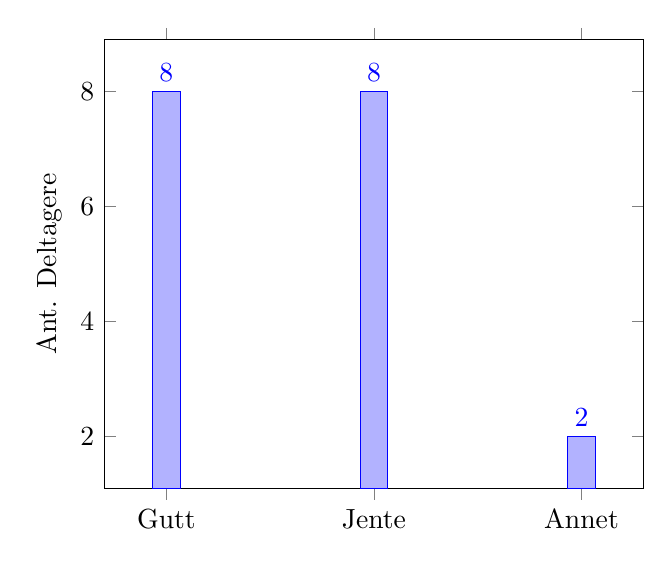
\begin{tikzpicture}
        \begin{axis}[ybar, enlargelimits=0.15, legend style={at={(0.5,-0.2)},
            anchor=north, legend columns=-1}, ylabel={Ant. Deltagere},
            symbolic x coords={Gutt, Jente, Annet}, xtick=data,
            nodes near coords, nodes near coords align={vertical},]
            % x tick label style={rotate=15, anchor=east},]
            \addplot coordinates {(Gutt, 8) (Jente, 8) (Annet, 2)};
        \end{axis}
    \end{tikzpicture}
    \caption{Test}
\end{figure}

\newpage